\chapter{Model predictive control}
\label{ch:mpc}
The objective of this investigation is to obtain a control signal for the heat pump of the reference building that considers grid services, occupancy comfort, and weather forecasts. Therefore, the suitable tool MPC is used. In this chapter, the framework conditions of the MPC are described by answering the questions: (i) What is controlled? (ii) How is it controlled? (iii) What is the desired output? (iii) What data is used? Additionally, the constraints, the cost function, and the workflow of the MPC script are introduced. In the present work, the controller is not applied to the real building, but is tested by simulation. \newline

\section{Framework conditions of the MPC}
\label{section:FrameworkMPC}
The objective of the MPC is to optimise the control signal of the reference building \newline $\mathbf{u} = (u_1 \enspace u_2)^T = (\dot{Q}_\text{heating} \enspace \dot{Q}_\text{HP})^T$. To this end, we consider the heat flows of the building in the MPC simulation. To investigate DSM, we want to achieve an impact of the control signal on the grid. Therefore, we calculate the electrical control signal $P_\text{HP}$ using the characteristic diagram of the heat pump from the optimised $\dot{Q}_\text{HP}$. The controlled output is the inside temperature $\mathbf{y} = T_\text{inside}$, which we calculate with the thermal model from \autoref{holeModel}. The desired trajectories of $\mathbf{y}$ depend on the presence of occupants, which is determined by an occupancy schedule. To obtain a simulation environment, we use past data of the weather as the disturbances $d_\text{k}$ and the dynamic price of the electricity $Pr$ \nomenclature[P]{Pr}{dynamic Price of the electricity } as an indicator for the grid balance. The characteristic diagram, the occupancy schedule, and the used data are introduced in the following subsections.    

\subsection{Characteristic diagram of the heat pump}
\label{subsec:charcteristicDiagramHP}
The characteristic diagram of the heat pump is interpolated from the characteristic values specified by the producer \cite{TUM}. We assume an operation at the nominal power of the heat pump. As \autoref{fig:HeatpumpKennfeld} shows, the electrical power $P_\text{HP}$ depends on the outside temperature $T_\text{outside}$ and the required heat flow $\dot{Q}_\text{HP}$. Further, the heat pump can generate negative heat flows when cooling is desired. The optimisation of the MPC computes $\dot{Q}_\text{HP}$, and $T_\text{outside}$ is known at every time step, hence the characteristics of the heat pump are used to calculate $P_\text{HP}$. Since the control signal is a heat flow, the effects on the grid cannot be assessed directly. Therefore, $P_\text{HP}$ is needed to analyse the effects on the grid. Furthermore, converting $\mathbf{u}$ into $P_\text{HP}$ simplifies the analysis, as we then only consider positive values.
    \begin{figure}[h]
            \centering
            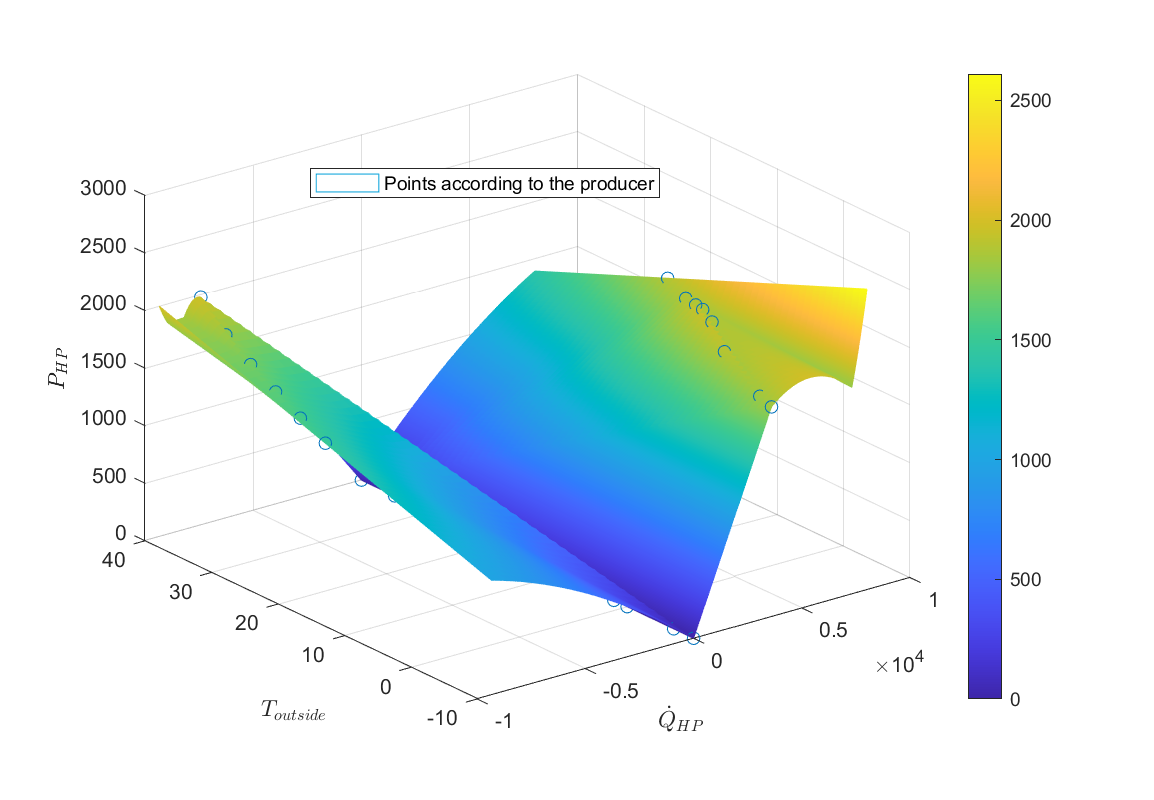
\includegraphics[width=8cm,height=6.5cm]{figure/HeatPumpV55nenn.eps}
           \caption{Interpolation of the characteristic diagram of the heat pump with nominal power according to \cite{TUM}}
           \label{fig:HeatpumpKennfeld}
    \end{figure}
    
\subsection{Occupancy schedule}
\label{subsec:OccupancySchedule}
Since the reference building is used as an office, the occupancy schedule describes at which day and time persons work in the reference building. We use the schedule as a specification when the comfort should be considered in the MPC. \autoref{fig:OccupancySchedule} shows the occupancy schedule. It summarises the working time of occupants with a green bar. We assume that persons are in the reference building from Monday to Thursday from 6 am to 7 pm and on Friday from 6 to 6 pm. The assumption is based on experience values and means that there is a high probability that persons will be in the building during this time.  
    \begin{figure}[H]
            \centering
            
\includegraphics[width=15cm]{figure/Occupancy schedule.PNG}
           \caption{Occupancy schedule of the reference building}
           \label{fig:OccupancySchedule}
    \end{figure}

\subsection{Used data}
\label{subsec:PastData}
    In a real world application of an MPC, we would use weather forecast as the disturbances $d_\text{k}$ in the state-space formulation for calculating the future behaviour of the system with the optimal control signal. Since we only simulate the behaviour of the building, we can use past data of the weather as $d_\text{k}$.\newline
    The data used is from the same period as the training data for the model estimation. As the disturbance variable, we use the recording of diffuse radiation and outside temperature in Energy Lab 2.0. The MPC is simulated over nine days, to consider the full occupancy schedule at least once.\newline
    The dynamic price of the electricity  $Pr$ is made available on the website of the Bundesnetzagentur \cite{Bundesnetzagentur-smard}. Here we use the wholesale prices on the stock exchange as an indicator of grid services. The price is formed by supply and demand. Consequently, when the price is low, we can assume an excess of electricity in the grid. Then it is particularly suitable to operate our heat pump to obtain electricity from the grid. In the opposite case, the same applies: If the price is high, it is unfavourable to operate the heat pump. At such times, it is particularly unsuitable to supply power from the grid. \newline
    However, negative prices can also arise in retail. Negative prices would undesirably change the cost function, which will be explained in detail later with reference to the cost function. To avoid negative prices, we add the absolute minimum value of $Pr$ to every value of $Pr$. Thus, we shift the curve of $Pr$ into positive and obtain as minimum $Pr = 0 \frac{\text{\euro}}{kWh}$ , as shown in \autoref{fig:Gridverschiebung}. Henceforth, we will utilise the dynamic price of electricity $Pr$ in the unit of $\frac{\text{\euro}}{Wh}$.
    \begin{figure}[h]
            \centering
            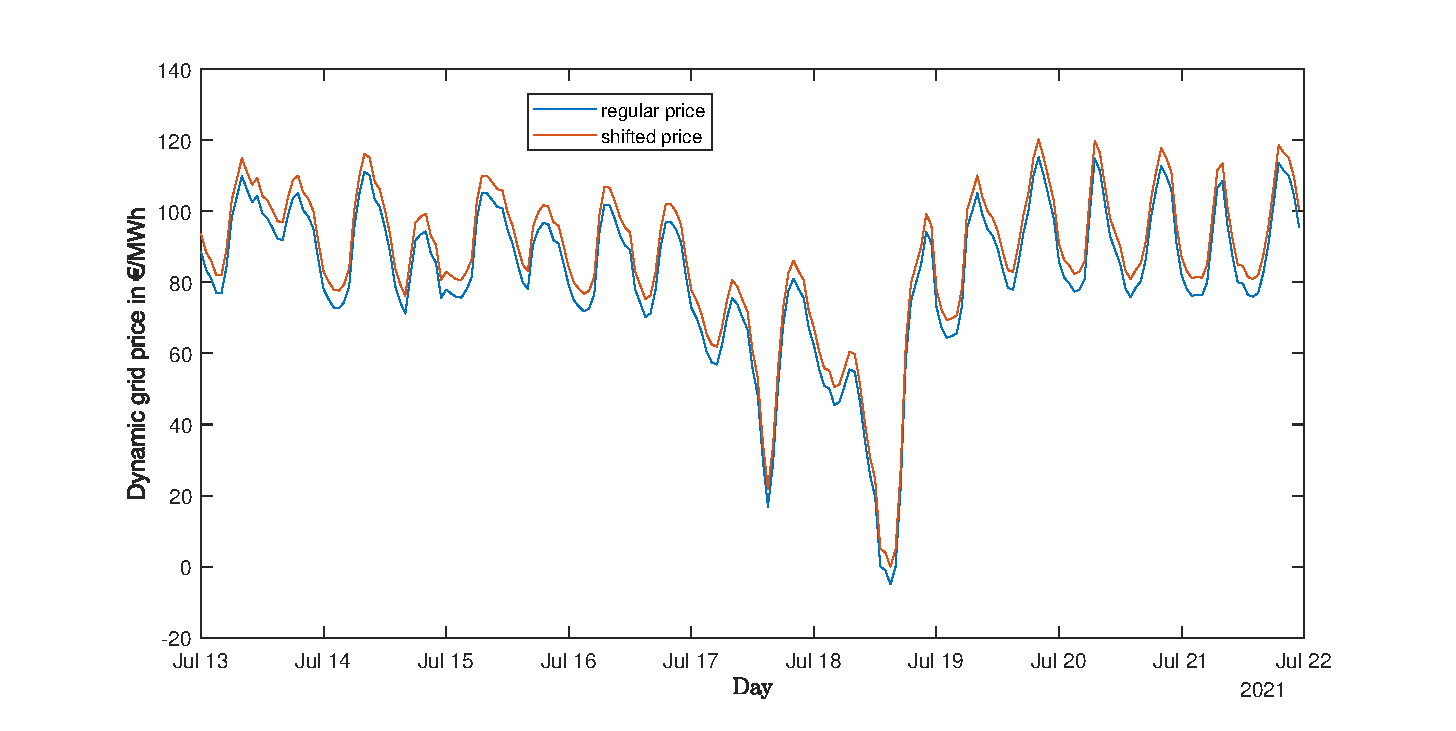
\includegraphics[width=15cm,height=8cm]{figure/Grid_data_Verschiebung.eps}
           \caption{Dynamic price of electricity \cite{Bundesnetzagentur-smard} and shifted dynamic price of electricity}
            \label{fig:Gridverschiebung}
    \end{figure}
    
\section{The Constraints}
\label{section:theconstraints}
We generally define in \autoref{subsection:constraints} constraints. Further, we differ soft and hard constraints in the following. The hard constraints depend on the physical limitations of the installations in the building, such as the heat pump, the underground floor heating, and the water reservoir. The used soft constraint in this MPC are smoothed constraints on the temperature range. Further, the integration method of the model is included in the constraints to calculate the future states over one horizon. The subsequent section gives an overview of the constraints regarding the control signal, the output, the states, and an introduction of the integration method.

\subsection{Constraints of the control signals}
\label{subsec:COnstraintU}
The control signals are constrained by the physical limitations of the heat pump, the underfloor heating and the cooling configurations.\newline
The producer's specifications restrict $\dot{Q}_\text{HP}$ for nominal power by an inlet temperature of 55°C in case of heating and by an inlet temperature of 18°C in case of cooling \cite{TUM}. The maximum $\dot{Q}_\text{heating}$ is limited according to the underground floor heating calculation, where the set power of every room is counted and summed for the complete building \cite{Roth_Auslegung.2020}. The computation of the required cooling power predicts 2246 W needed power in case of 34.5°C outside temperature in July \cite{SEFIngenieurgesellschaftMBH.2019}. To be more flexible with higher outside temperatures, we round the minimum $\dot{Q}_\text{heating}$ to 2300 W.\newline
Further, we define a constraint $u_1 \cdot u_2 \geq 0$ to avoid simultaneous heating of building and cooling of the water reservoir or reversed as this would waste energy needlessly.
The set $\mathbb{U_k}$ summarise mathematically the constraints.
\begin{equation}
    \label{ConstraintU}
    \mathbb{U_k} = \{\mathbf{u_k}| -2300 W \leq \dot{Q}_\text{heating} \leq 5283 W \wedge -9340 W \leq \dot{Q}_\text{HP} \leq 8010 W | u_1 \cdot u_2 \geq 0\} 
\end{equation}

\subsection{Constraint of the output}
\label{subsec:constrainY}
We specify a comfortable temperature range with a soft constraint of the output. The following explains the range of a comfortable temperature.\newline
The Umweltbundesamt \cite{Umweltbundesamt.7.10.2021} recommends an inside temperature of 18°C as comfortable temperature for some rooms, such as the kitchen. We expand the recommendation to a minimum $T_\text{inside}$ of 18°C for all rooms. The maximum inside temperature refers to the German technical rules for workplaces \cite{Bund.2021}, wherein a maximum of 26°C as room temperature is prescribed. The slack variable $\eta_\text{k}$ allows a variance of the given temperature range with a simultaneous penalty in the cost function. Thus, we have a soft constraint, and we can maintain the feasibility of the optimisation problem during a deviation of the temperature range \cite{Drgona.2020}. The constraint is represented by the set $\mathbb{Y_k}$ as follows:  
\begin{equation}
    \label{ConstraintY}
    \mathbb{Y_k} = \{\mathbf{y_k}| 18 \text{°C} - \eta_k \leq T_\text{inside} \leq 26 \text{°C}+ \eta_k\} 
\end{equation}

\subsection{Constraints on the states}
\label{ConstraintX}
We only have to constrain the state of the water reservoir because of its physical limitation. Therefore, we use a hard constraint.
The calculation of the water reservoirs maximal inner energy $U_\text{WR}$ is explained in \autoref{waterModel} with \autoref{eq:max.Energie}. The minimum $U_\text{WR}$ is 0 J. The set $\mathbb{X}_{5,k}$ describes the constraint for the fifth element of the state vector.
\begin{equation}
    \label{ConstraintX5}
    \mathbb{X}_{5,k} = \{x_\text{5,k}| 0 J \leq U_\text{WR} \leq 96370000 J\} 
\end{equation}
A further constraint, which relates to the states, is the integration method as discussed below.

\subsection{Integration method and the corresponding constraint}
\label{COnstaintIntegration}
As an integration method, we use an explicit single-step method, which means that we only need the values of the current time step $k$ to compute the next. Possible methods are the Heun's method, the Euler and the Runge-Kutta method. The decision is made in favor of the fourth-order Runge-Kutta method because the fourth order makes it more precise at a given step size than the other methods mentioned above. The following equation shows the integration scheme using the Runge-Kutta method with the sample time $T_\text{s}$ and the function $f(\mathbf{x_k},t_\text{k},\mathbf{u_k},\mathbf{d_k}) = \mathbf{\dot{x}_\text{k}}$ according the state-space formulation (see \autoref{eq:statespace}) \cite{KaiFurmansMarcusGeimerBalazsPritzCarstenProppe.WS1920}.

    \begin{align}
        \label{Runke-Kutta}
        a_k^{(1)} = T_s \cdot f(\mathbf{x_k},t_\text{k},\mathbf{u_k},\mathbf{d_k}) \\
        a_k^{(2)} = T_s \cdot f(\mathbf{x_k}+\frac{a_k^{(1)}}{2},t_k+\frac{T_s}{2},\mathbf{u_k},\mathbf{d_k})\nonumber\\
        a_k^{(3)} = T_s \cdot f(\mathbf{x_k}+\frac{a_k^{(2)}}{2},t_k+\frac{T_s}{2},\mathbf{u_k},\mathbf{d_k})\nonumber\\
        a_k^{(4)} = T_s \cdot f(\mathbf{x_k}+a_k^{(3)},t_k+T_s,\mathbf{u_k},\mathbf{d_k})\nonumber\\
        \nonumber\\
        \mathbf{x_{k+1}} = \mathbf{x_k} + \frac{1}{6}\cdot (a_k^{(1)} + 2 a_k^{(2)} + 2 a_k^{(3)} + a_k^{(4)})\nonumber
    \end{align}
The constraints accommodate the integration method for calculating the next time step according to the determined thermal model.
Important to note is that the time step of the integration is chosen in accordance with the discretization of the model. The model is estimated with the discrete values of the reference building, where the measuring points are sampled every two minutes. For example, to achieve a $T_\text{s}$ of one hour, $T_\text{s}$ is described as $30 \cdot 2 min$. The two minutes are already included in the model by estimation. Therefore, we multiply $\mathbf{\dot{x}_\text{k}}$ by 30 to go one time step by one hour further. It is considered that the thermal model is composed of two submodels. The water reservoir sub-model, which is modelled using the white-box approach, requires a different conversion to advance one hour. Here we convert watts to joules per hour. In the MPC, this difference is compensated by a factor directly in the state-space formulation of the model.

\section{The Cost function}
\label{section:thecostfunction}

The cost function penalises the deviation from the desired requirements. On the one hand, we have to guaranty thermal occupant comfort in the building. On the other hand, we prefer to heat with the heat pump when grid service is favourable. Both subjects are represented in the cost function below with the weightings $w_\text{1}$ and $w_\text{1}$, which relate to the requirements comfort and grid services.
    \begin{equation}
        \text{minimize} \sum_{k} w_\text{1}\cdot (y_\text{k}-y_\text{track})^2 + w_\textbf{2}\cdot(u_\text{2,k}\cdot Pr_\text{k})^2 + w_\text{3} \cdot \eta_\text{k}^2
        \label{eq:costfunctatsächlich}
    \end{equation}
At first, we determine the desired temperature $y_\text{track}$ of the comfort requirement in the cost function. A pleasant air temperature is 22°C for living rooms, working rooms, and the bathroom \cite{Umweltbundesamt.7.10.2021}. As discussed in \autoref{ch:modelling}, we model the reference building as a single-zone building, wherein most rooms are working rooms. We decide to use the median temperature of all rooms of the recommended temperatures for the complete building. Thus, the desired temperature is $y_\text{track} = 22$°C.\newline
The expression $(y_\text{k}-y_\text{track})^2$ represents the comfort requirement in the cost function. The squaring of $(y_\text{k}-y_\text{track})$ avoid a minimising of the cost function due to negative $(y_\text{k}-y_\text{track})$ values. The same is applied to the expression of the grid service $(u_\text{2,k}\cdot Pr_\text{k})^2$. We exclude negative values of $Pr_\text{k}$ (as explained in \autoref{subsec:PastData}) because they would generate an incorrect effect. Then after squaring, the expression $(u_\text{2,k}\cdot Pr_\text{k})^2$ would maximise the cost function during a appropriate time for grid services due to a negative $Pr_\text{k}$. Without a squaring, we would support energy consumption while its not needed or we would penalise a cooling by we having a negative $u_\text{2,k}$ multiplied with a negative $Pr_\text{k}$.\newline
We can adjust the preference of the requirements comfort and grid services by the weightings $w_\text{1}$ and $w_\text{2}$. How much deviation is allowed from the temperature range in the soft constraint is determined by the weighting $w_\text{3}$.\newline
The magnitude of the costs of the requirements are different. When considering the constraints, $y_\text{k}-y_\text{track}$ can reach a maximum deviation of 4 K (without soft constraint), while $u_\text{2,k}\cdot Pr_\text{k}$ is in a lower order of magnitude due to the unit $\frac{\text{\euro}}{Wh}$. To compensate for this, a factor is introduced that gives the comfort requirement a weaker weighting in the cost function. The factor is integrated into the weighing $w_\text{1}$ as shown in the following table. In general, we vary the weights $w_\text{1}$ and $w_\text{2}$ of the cost function from $ i_{1}= 0$ to 1 in steps of 0.1. As shown in table \autoref{tab:weighting factor}, the comfort with $w_\text{1}$ and the grid service with $w_\text{2}$ are always weighted in opposite directions.\newline
\begin{table}[h]
    \centering
    \begin{tabular}{c|c|c}
         $w_\text{1}$ & $w_\text{2}$ & $w_\text{3}$ \\
        $\frac{1}{4} \cdot i_\text{1}$ & $i_\text{2}=1-i_\text{1}$ & 0.01
    \end{tabular}
    \caption{Weighting factor}
    \label{tab:weighting factor}
\end{table}
Occupant comfort is only necessary if persons are present in the building. Therefore, we consider the cost function during absence without the comfort requirement by setting $w_\text{1}$ to zero according to the occupancy schedule, which results in the following simplification of the cost function during absence.
    \begin{equation}
        \text{minimize} \sum_{k=1}^{N-1} w_\textbf{2}\cdot(u_\text{2,k}\cdot Pr_\text{k})^2 + w_\text{3} \cdot \eta_\text{k}^2
        \label{eq:costfunctionAbwesenheit}
    \end{equation}
The procedure aims to generate more flexibility for the objective of grid services. We define this scenario with the changing cost function as the basic scenario for this thesis, which is needed in the following chapter. 

\section{Workflow of the MPC script}
\label{section:workflowMPC}
The approach in the MPC script is determined by the use of the tool CasAdi. CasADi is an open-source tool for nonlinear optimisation and algorithmic differentiation and is characterised by a symbolic framework. Optimal control problems, such as an MPC, are of particular interest \cite{JoelA.E.Andersson.2018}. We can combine CasAdi with MATLAB through a simple import.\newline
\autoref{fig:workflowMPC} gives an overview of the workflow of the MPC script. First, we declare the parameter, all known dimensions, and the optimisation variables symbolically. Then the inequalities of the constraints are set in a loop over the prediction horizon with the symbolic variables. The cost function is also indicated symbolically for the horizon. Afterwards, the initial values for the optimiser are determined. To specify the initial state for the first MPC step, we choose a constant control signal $\mathbf{u_k} = [0\enspace0]^T$, a state $\mathbf{x}$ within the temperature range, and determine with the Runge-Kutta method the trajectory over the horizon. A half charged water reservoir constitutes a further assumption for the initial state. We pass the values of the initial state of the optimisation variations and the parameters to the solver. Then, the optimisation problem is solved with the Ipopt (\textbf{I}nterior \textbf{P}oint \textbf{Opt}imiser) solver \cite{JoelA.E.Andersson.2018}. As a result, we obtain the optimised $\mathbf{u_k}$ over the horizon. Now, after each time step, a new initial state is calculated with the curves of the states and the output from the new disturbance variables and the optimum $\mathbf{u_k}$ over the horizon before.
    \begin{figure}[h]
            \centering
            \def\svgwidth{0.75\textwidth}
            \input{figure/workflowMPC2.pdf_tex}
            \caption{Workflow of the MPC script}
            \label{fig:workflowMPC}
    \end{figure}
    
\section{Choice of weightings and horizon}
\label{Choise of weigtings and horizon}
In the following, we analyse the horizon length $N$ \nomenclature[P]{N}{Length of the predictive horizon} and the effects of the weightings on the requirement of occupancy comfort and grid services for the basic scenario. For a better comparison we define an average comfort $\Delta \overline{y}$ \nomenclature[P]{$\Delta \overline{y}$}{Average comfort}, which is the average deviation of $y$ from $y_\text{track}$ over the simulation time only during presence of occupants, expressed by $y_\text{k,occ} - y_\text{track}$. The calculation of $\Delta \overline{y}$ is described in the following equation with the number of time steps with occupants $n_\text{occ}$.
\begin{equation}
    \label{eq:average comfort}
    \Delta \overline{y} = \frac{\sum_{k,occ}^{n_\text{occ}} |y_\text{k,occ} - y_\text{track}|}{n_\text{occ}}
\end{equation}
On the other hand, we define the costs for grid services (GS) \nomenclature[A]{GS}{Costs for grid services} over the whole simulation time (with the number of time steps $n$) as the sum of the electrical power of the heat pump $P_\text{HP,k}$ multiplied with the dynamic price of electricity $Pr_\text{k}$:
\begin{equation}
\label{eq:GridService123}
    GS = \sum_{k}^n P_{HP,k}\cdot Pr_\text{k}
\end{equation}
In theoretical considerations, we should obtain a higher value of $\Delta \overline{y}$ with less weighting of comfort and a higher value of GS with less weighting of grid services. Furthermore, a larger or shorter horizon $N$ differs in computation time and finding the optimal solution in comparing with the same sample time. While a longer N requires more computation time and may not find a solution, a shorter $N$ find only the optimal solution over the short horizon neglecting later influences. Therefore, a larger horizon should result in less costs for the requirements over the simulation period because of including later influences. In general, the horizon should be long enough to detect early deviations from the constraints \cite{Dittmar.2019}. \newline
The theoretical considerations are inspected in the subsequent sections for the basic scenario over the simulation time of nine days.   

\subsection{Average comfort and grid services over the weightings}
\label{subsec:Average comfort and grid services over the weightings}
The following figure presents the behaviour of $\Delta \overline{y}$ and GS for the different weightings $w_\text{1}$ and $w_\text{2}$ with $N = 24h$. We also compare the behaviour for different horizons $N$ to verify the feasibility and the expected behaviour. The corresponding figures are shown in \autoref{sec:Average comfort and grid services} and the values of $\Delta \overline{y}$ and GS for different horizons are displayed in the following tables.\newline
We notice a monotone behaviour of the average comfort and the grid services according to their weightings apart from small discrepancies. A possibility for discrepancies could be that the optimiser find not the global optimum. We obtain feasible solutions apart from $N=12 h$ and both weightings are $0.5$. The lower costs with increasing horizon length are only for the average comfort notable, expecting the case $w_\text{1}=0$. In this case, we consider not the comfort in the cost function. Therefore, the values of $\Delta \overline{y}$ are random, also relating to the horizon length.\newline
The explanation for higher cost in GS with longer horizon is that the thermal reaction of the building is known over a longer time and the control signal reacts early for a better adaption of the comfort.
    \begin{figure}[h]
            \centering
            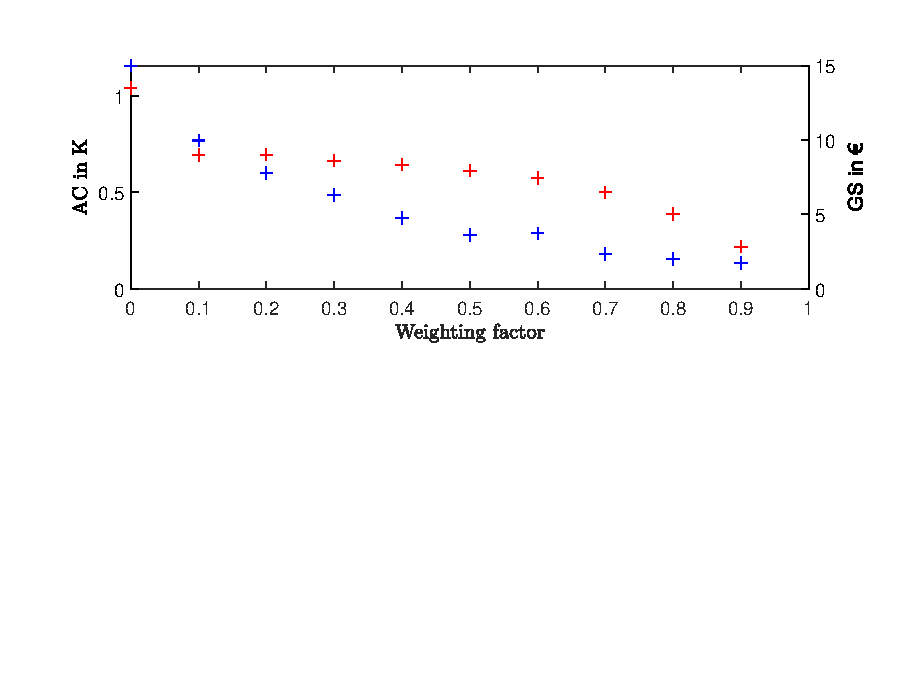
\includegraphics[width=15cm,height=8cm]{figure/AC_und_GS_24h.eps}
           \caption{$\Delta \overline{y}$ and GS for N = 24h}
            \label{fig:AC_und_GS_24h}
    \end{figure}
    
    \begin{table}[H]
    \centering
    \begin{tabular}{c|c|c|c|c|c|c|c|c|c|c|c}
         weighting factor i&0&0.1&0.2&0.3&0.4&0.5&0.6&0.7&0.8&0.9&1  \\
         \hline
         $\Delta \overline{y}$ by N = 12 h& 1.11 & 0.89 & 0.77 & 0.64 & 0.54 &  & 0.40 & 0.28 & 0.24 & 0.22 & 0.22\\
         $\Delta \overline{y}$ by N = 18 h& 1.14 & 0.80 & 0.72 & 0.54 & 0.43 & 0.35 & 0.41 & 0.24 & 0.17 & 0.16 & 0.14\\
         $\Delta \overline{y}$ by N = 24 h&  1.16 & 0.77 & 0.60 & 0.49 & 0.37 & 0.28 & 0.29 & 0.18 & 0.15 & 0.14 & 0.20\\
         $\Delta \overline{y}$ by N = 30 h& 1.16 & 0.75 & 0.55 & 0.42 & 0.31 & 0.25 & 0.22 & 0.18 & 0.16 & 0.14 & 0.16\\
    \end{tabular}
    \caption{$\Delta \overline{y}$ for different N}
    \label{tab:AC for different N}
    \end{table}
    
    \begin{table}[H]
    \centering
    \begin{tabular}{c|c|c|c|c|c|c|c|c|c|c|c}
         weighting factor i&0&0.1&0.2&0.3&0.4&0.5&0.6&0.7&0.8&0.9&1  \\
         \hline
         GS by N = 12 h& 11.97 & 8.31 & 7.90 & 7.35 & 6.93 &  & 5.23 & 4.37 & 3.12 & 1.71 & 0.00\\
         GS by N = 18 h & 16.45 & 9.16 & 8.76 & 8.57 & 7.61 & 7.57 & 6.77 & 5.68 & 4.05 & 2.39 & 0.00\\
         GS by N = 24 h & 13.50 & 9.00 & 9.01 & 8.62 & 8.35 & 7.94 & 7.44 & 6.49 & 5.03 & 2.85 & 0.00\\
         GS by N = 30 h & 13.74 & 8.82 & 8.81 & 8.56 & 8.65 & 8.13 & 7.48 & 6.62 & 5.28 & 3.39 & 0.00\\
    \end{tabular}
    \caption{GS for different N}
    \label{tab:GS for different N}
\end{table}
    
\subsection{Choice of the horizon}
\label{subsec:ChoiceHorizon}
A predictive horizon should depict the dynamics of the system, in this case, the temperature profile inside the reference building. Therefore, the following figure shows $T_\text{inside}$ of the building over three days determined from the measurements as a single-zone building as explained in \autoref{ch:modelling}. We notice around every 24 h a periodic wave in the temperature profile, which is highlighted with vertical lines.\newline
    \begin{figure}[H]
            \centering
            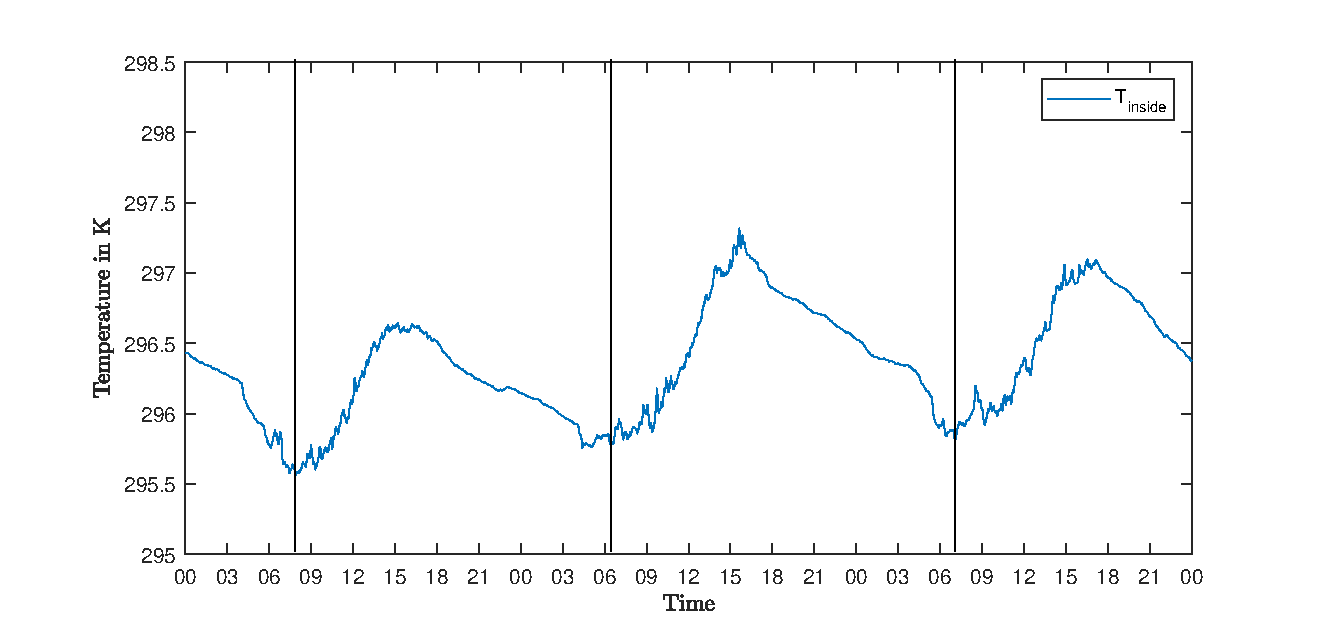
\includegraphics[width=15cm,height=5cm]{figure/Plot_T_inside_Prediction_zeigen.eps}
           \caption{Measured data of the reference building: $T_\text{inside}$ over three days}
            \label{fig:Plot_T_inside_Prediction_zeigen}
    \end{figure}
The wavy profile occurs by day and night fluctuations of the weather. Therefore, \autoref{fig:Plot_T_inside_Prediction_zeigen} seems to be an indicator for the dynamics of the system, but the reaction of $T_\text{inside}$ to a control signal is not illustrated. Nevertheless, we propose a predictive horizon of one day in order to consider complete day and night fluctuations in the predictions. We examine this consideration by comparing costs over different horizons for an exemplary weighting. The following figure shows the curve of costs over the simulation period. The costs here are the sum of comfort and grid services. Here, the comfort according to the occupancy schedule is only considered when the occupants are in the building. Therefore, the peaks are recognizable, and from day four to the beginning of six, there are almost no costs, as this is the weekend.
    \begin{figure}[H]
            \centering
            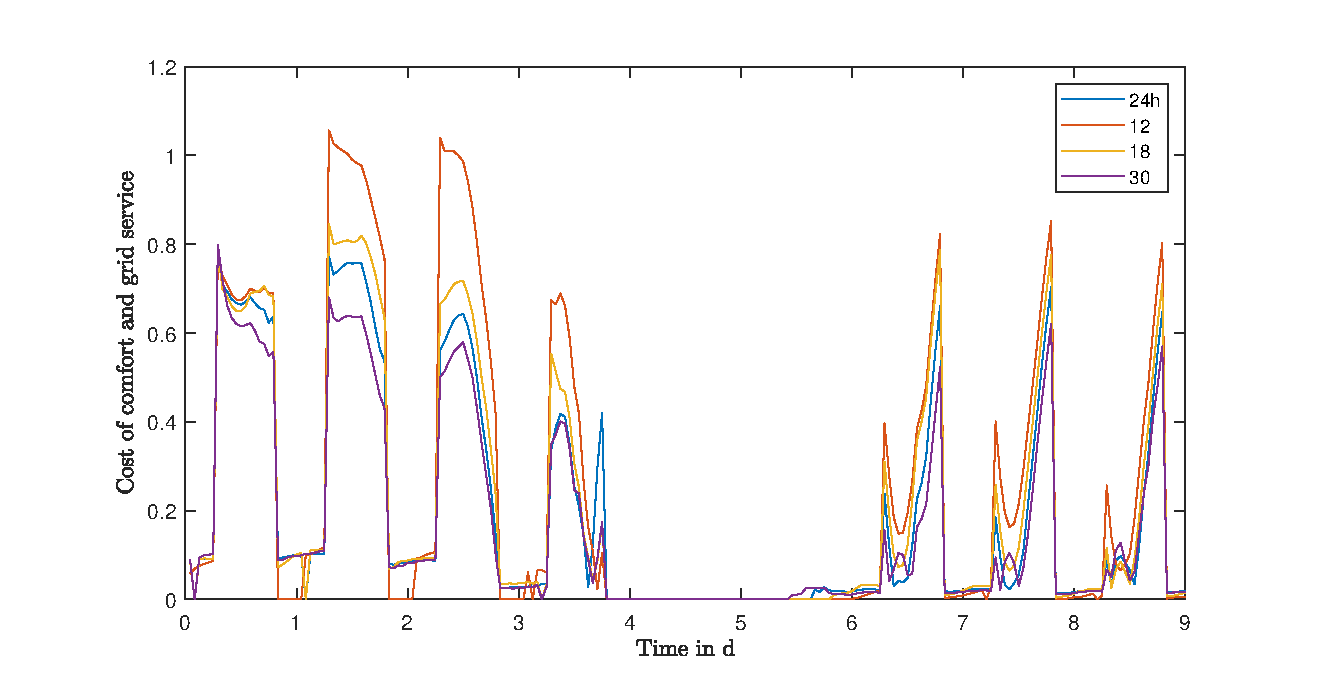
\includegraphics[width=15cm,height=5cm]{figure/Gesamtkosten_Vergleich_horizonte.eps}
           \caption{Curve of the sum of cost over simulation time for different $N$}
            \label{fig:Gesamtkosten_Vergleich_horizonte}
    \end{figure}
The distinctions in costs at different horizons are as expected. The horizon $N = 12 h$ has the highest costs, while with the longer predictions, the costs decrease.\newline 
We choose the horizon of 24 h because it represents the dynamic of the reference building and the costs are partly very similar to the next longer horizon of 30 h, e.g. in the last simulation days.

\section{Mathematical description of the MPC}
\label{sec:mathematicalDescriptionMPC}
The following equation summarises mathematically the above explained MPC according to the foundations from \autoref{section:mpc}. Comparing the foundations and \autoref{eq:MPCsum}, it is notable that here the cost function from \autoref{section:thecostfunction}, the constraints from \autoref{section:theconstraints} and the determined predictive horizon $N = 24h$ is depicted, furthermore $f(\mathbf{x_k},t_\text{k},\mathbf{u_k},\mathbf{d_k}) = \dot{x}_\text{k}$ according to \autoref{eq:ZRD Modell} and $g(\mathbf{x_k})$ corresponds to \autoref{y}.  
\begin{align}
\label{eq:MPCsum}
\textrm{Cost function} && \text{minimize} \sum_{k} w_\text{1}\cdot (y_\text{k}-y_\text{track})^2 + w_\textbf{2}\cdot(u_\text{2,k}\cdot Pr_\text{k})^2 + w_\text{3} \cdot \eta_\text{k}^2
\end{align}
subject to 
\begin{align*}
\forall k \in [0,24-1]\\
\textrm{Current state} && \mathbf{x_0} = \mathbf{x} \\	
\textrm{Dynamics} && a_k^{(1)} = T_s \cdot f(\mathbf{x_k},t_\text{k},\mathbf{u_k},\mathbf{d_k}) \\
        && a_k^{(2)} = T_s \cdot f(\mathbf{x_k}+\frac{a_k^{(1)}}{2},t_k+\frac{T_s}{2},\mathbf{u_k},\mathbf{d_k})\\
        && a_k^{(3)} = T_s \cdot f(\mathbf{x_k}+\frac{a_k^{(2)}}{2},t_k+\frac{T_s}{2},\mathbf{u_k},\mathbf{d_k})\\
        && a_k^{(4)} = T_s \cdot f(\mathbf{x_k}+a_k^{(3)},t_k+T_s,\mathbf{u_k},\mathbf{d_k})\\
        \\
        && \mathbf{x_{k+1}} = \mathbf{x_k} + \frac{1}{6}\cdot (a_k^{(1)} + 2 a_k^{(2)} + 2 a_k^{(3)} + a_k^{(4)})\\
&&	\mathbf{y_k} = g(\mathbf{x_k})\\				
\textrm{Constraints} && x_\text{5,k} \in \mathbb{X}_{5,k} \\		
 && \mathbf{y_k} \in \mathbb{Y_k}\\
 && \mathbf{u_k} \in \mathbb{U_k}\\
\end{align*}